\documentclass[../DCM2_Verslag.tex]{subfiles}
\begin{document}

\section{Samenvatting package size testen}
De resultaten van de package size testen vertellen veel over de performance van de tcp/ip stack op de ESP32. Zo is er af te leiden dat bij het ontvangen een hoge package size wenselijk is. En bij lage package sizes de performance zwaar negatief wordt beinvloedt. De factoren die leiden tot deze negatieve beinvloeding zijn:\\\\ \-/ Overhead door de grote hoeveelheid kleine paketten die elk een TCP en IP header meedraagt tot de eindbestemming.\\
\-/ De tijd benodigt om de paketten te encapsuleren en decapsuleren.
\\\\
\clearpage
\subsection{Overhead}
Om te berekenen hoeveel overhead er is bij een 200 bytes package size t.o.v. 1400 bytes met een data grootte van 5Kb wordt er gebruik gemaakt van dit diagram:\\
\begin{figure}[h]
\centering
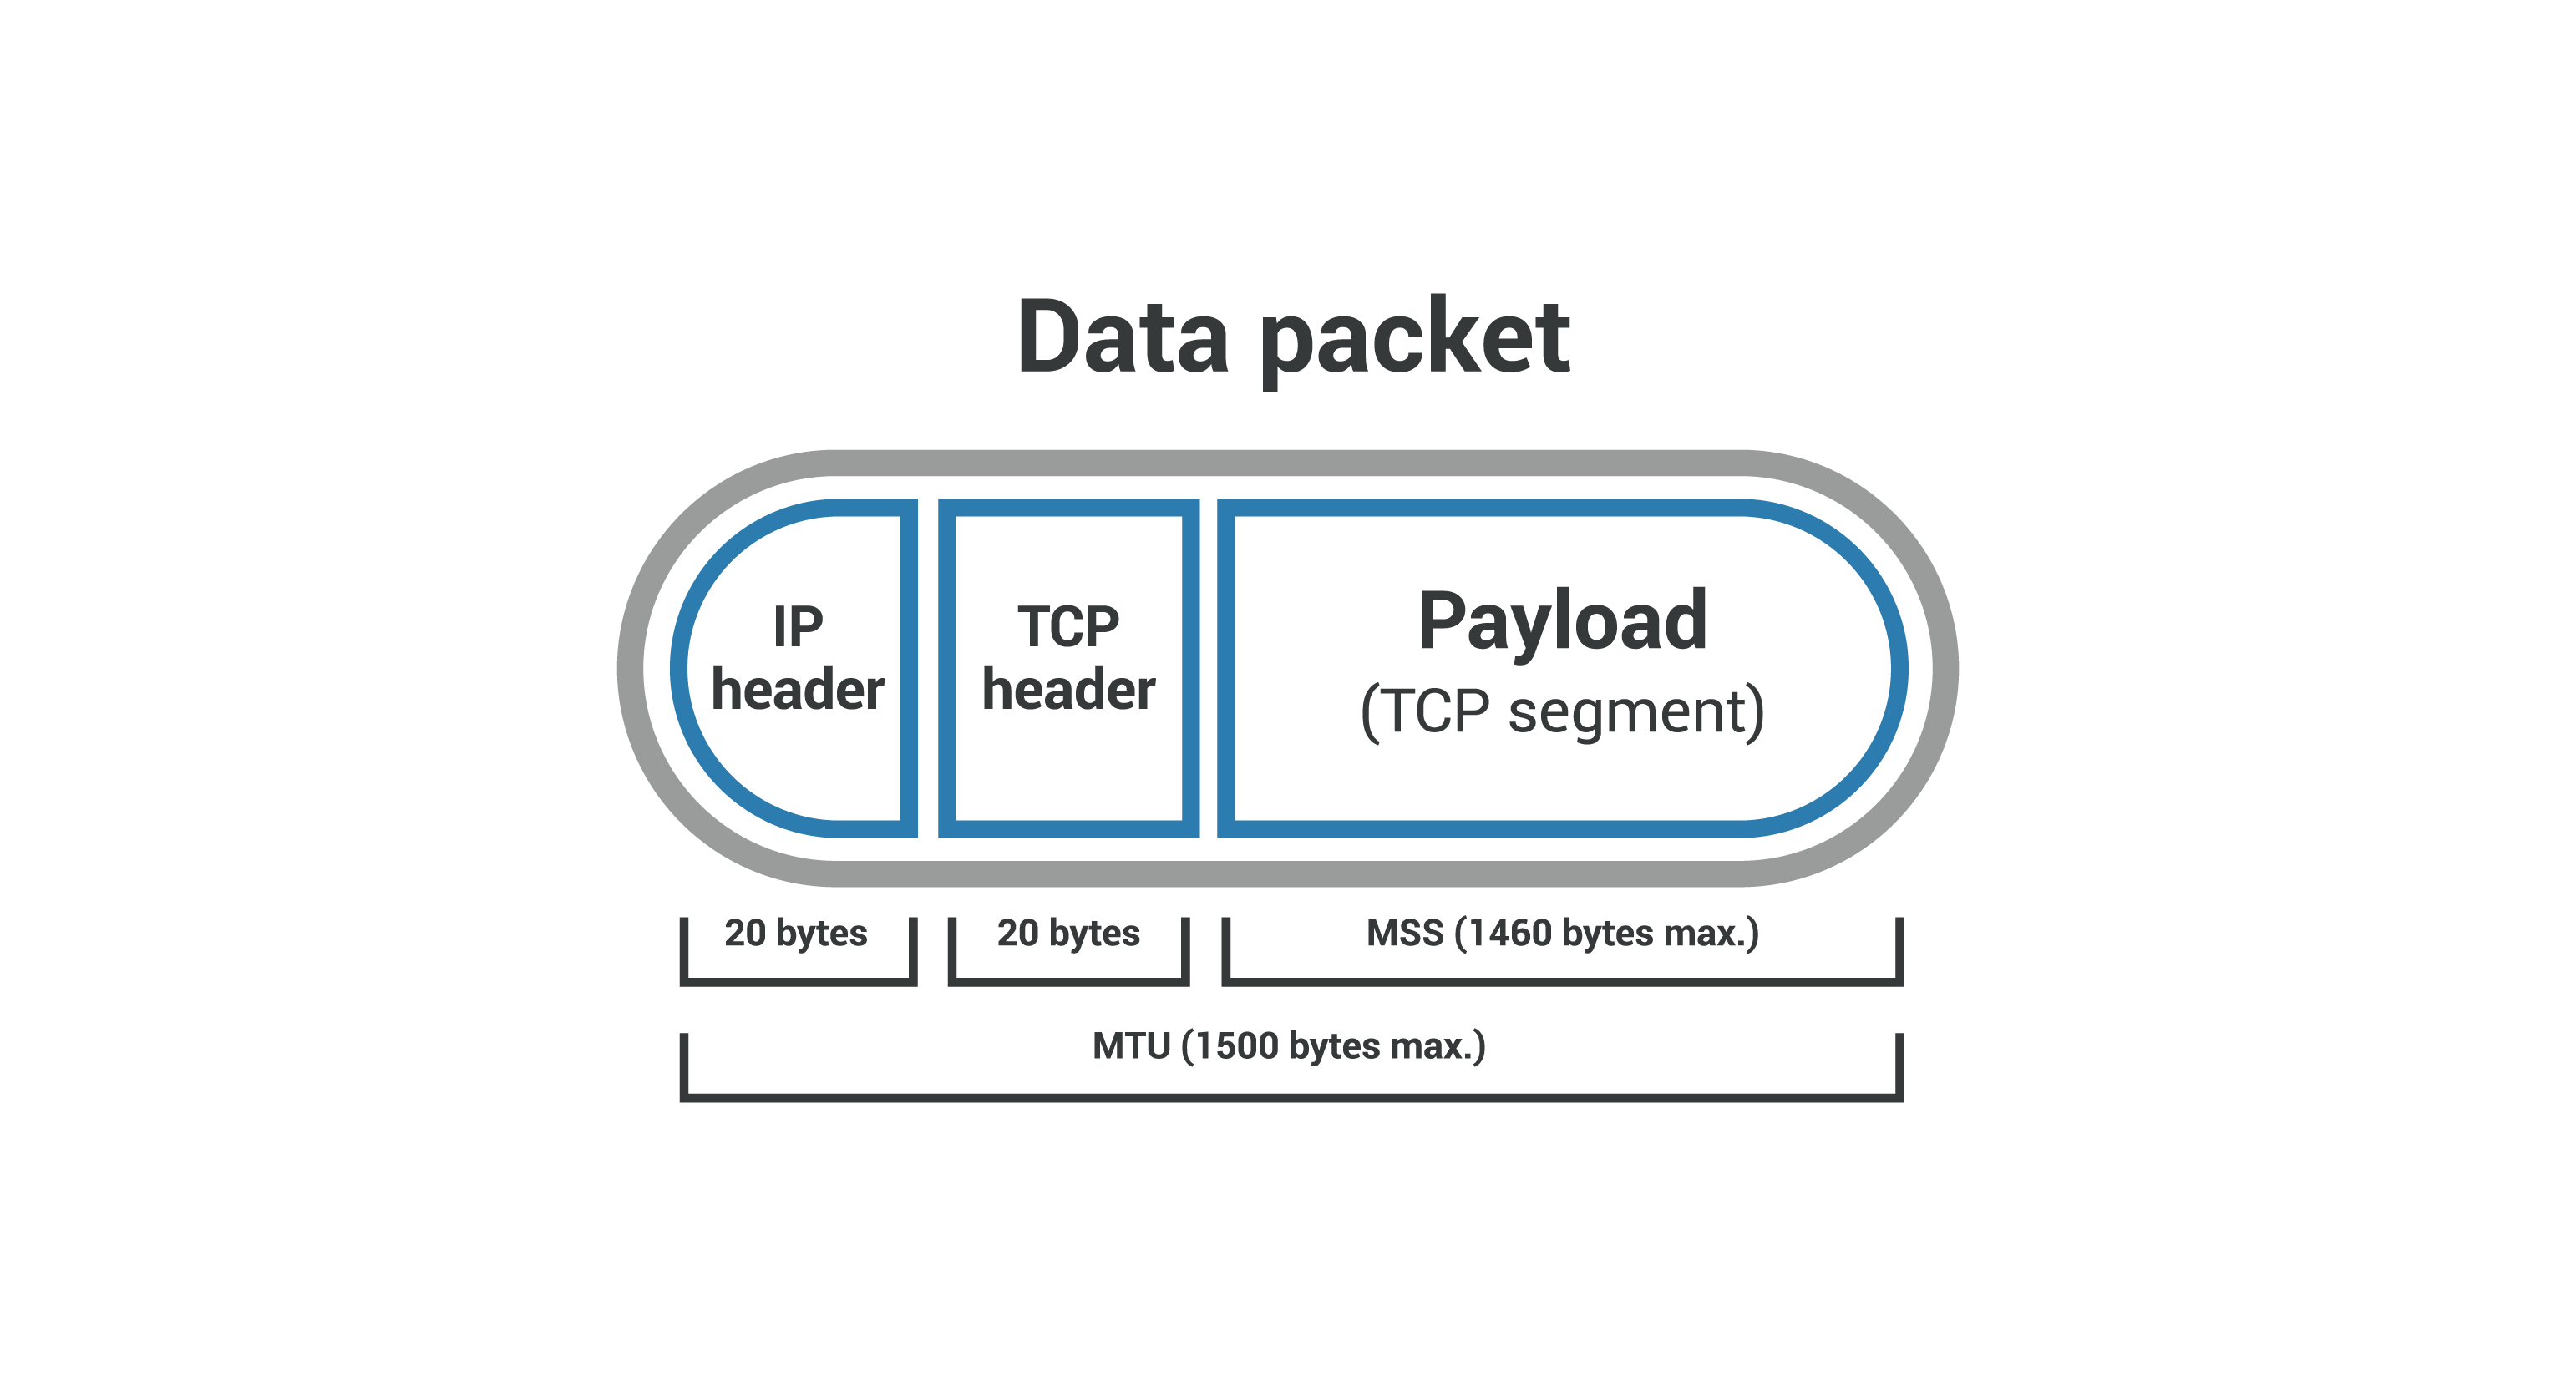
\includegraphics[scale=0.1]{MSS_TCP_segment_packet_diagram}
\caption{TCP/IP model}
\end{figure}
\\
Uit dit diagram is duidelijk dat er per pakket al 40 bytes aan TCP en IP headers mee wordt gestuurd. Dan is hier al uit af te leiden dat voor het kleine pakket een overhead is van:
\[Overhead_{200bytes} = (\lceil{\frac{N_{bytes}}{P_{size}}} * 40) =  (\frac{5000}{200}*40)= 1000 bytes\]
\[Overhead_{1400bytes} = (\lceil{\frac{5000}{1400}}*40)= 160 bytes\]
\\
De minimale overhead bij het gebruik van een package size van 200 bytes bij het versturen van 5 Kbytes is 840 bytes t.o.v. de grootst geteste package size. Dit creert een significante hoeveelheid overhead op de verbinding. Deze headers en data moeten verzameld worden, ingepakt (geencapsuleerd), verzonden, uitgepakt(gedecapsuleerd) en (de data zelf) gereconstrueerd. Hoe meer van de pakketten hoe vaker deze taken opnieuw uitgevoerd moeten worden.
\clearpage
\subsection{Encapsulatie en Decapsulatie}
Encapsulatie is het process van het insluiten van een hogere laag protocol in een lagere laag protocol. Encapsulatie gebeurt in de lagen waarbij de informatie van de laag erboven ingepakt wordt in een nieuw pakket met de informatie van de huidige laag. Dit pakket wordt weer doorgegeven naar de laag eronder. Dit blijft zich herhalen tot het bij de fysieke laag komt. Nadat de fysieke laag gepasseerd is, wordt het pakket verstuurd over het medium.\\\\
Decapsulatie is het uitpakken van een hogere laags protocol uit een lagere laag protocol. Het kan ook wel omgekeerde encapsulatie genoemd worden.\\\\
Het telkens opnieuw inpakken van paketten neemt veel processor en geheugenkracht in beslag, dit effect speelt een rol in de testresultaten.
\subsection{Optimale package size}
Uit de testen is gebleken dat er een optimale package size is voor de ESP32. De meest optimale package size is 1400 bytes voor ontvangen en 600 bytes voor het verzenden van data. 

\section{Maximale bitrate}
De maximale bitrate was ook een deelvraag. De hoogste bandbreedte van de resultaten waren bij de baseline testen met 56.83 Mbits/sec voor verzenden en 49.63 Mbits/sec voor ontvangen. Voor pakketten houd dit in dat het een bitrate van \[ 56.83 \cdot 10^{6}\] en \[49.63 \cdot 10^{6} \] bits per seconden. Voor de data die ontvangen en verzonden was: \\MSS van 1400 bytes, vast header formaat van 40-bytes in 1 seconde:\\
\[Data_{send1s} = N_{bytes -(\lceil{\frac{N_{bytes}}{P_{size}}} * 40)} =   56.83 \cdot 10^{6}\ - (\frac{ 56.83 \cdot 10^{6}}{1400}*40) = 56789407 bytes\]
\[Data_{recv1s} = N_{bytes -(\lceil{\frac{N_{bytes}}{P_{size}}} * 40)} =   49.63 \cdot 10^{6}\ - (\frac{ 49.63 \cdot 10^{6}}{1400}*40) = 48212000 bytes\]

\section{Voor welk doeleind is deze performance geschikt}
De performance die behaald is in de testen is vrij hoog voor een embedded systeem. De verbinding is dusdanig hoog dat het videobellen, audiobellen, videoplayback en audioplayback ondersteund. Bestanden van een paar Mb kunnen ook zonder problemen in vrij korte tijd gedownload worden op deze verbinding. Maar het is hoogstonwaarschijnlijk dat dit het doel was van het bedrijf Espressif toen de ESP32 op de markt werd gebracht. Het doeleind volgens de tech reference manual van de ESP32 \parencite{esptechref} is de IOT markt. De IOT markt staat vooralsnog bekend als een markt waar het downloaden en uploaden van kleine hoeveelheden data de norm is (<1 Kbyte normaal gesproken).

\clearpage
\section{Algemene Conclusie}
Het uitgevoerde onderzoek heeft een aantal dingen aan het licht gebracht. Zo is te concludereren dat de ESP32, ongeacht de package sizes, window sizes of protocol een hogere bandbreedte heeft met het verzenden (TX) dan het ontvangen (RX). \\\ Bovendien is te concluderen dat de ESP32 optimale window en package sizes heeft waarbij de bandbreedte het hoogst is. De optimale window en package size is dan wel weer afhankelijk van verzenden of ontvangen. Bij ontvangen zijn grotere window en package sizes gewenst en bij verzenden kleinere.


\end{document}
